\begin{center}
    \textbf{BAB III \\ PELAKSANAAN KERJA MAGANG}
    \addcontentsline{toc}{section}{BAB III PELAKSANAAN KERJA MAGANG}
\end{center}
\setcounter{section}{3}
\setcounter{subsection}{0}
\setcounter{figure}{0}

\subsection{Kedudukan dan Koordinasi}

Kedudukan penulis ditugaskan oleh perusahaan untuk menjadi web developer yang bertujuan 
untuk melakukan pembuatan \emph{website} profil perusahaan sebagai media atau sarana untuk marketing.

Dalam perusahaan ini, penulis memberikan didamping oleh komisaris (commissioner) 
yang bertindak sebagai business development yang bertujuan untuk memberikan ide, 
masukan dan selain itu memonitor pekerjaan dan arahan dari direktur dalam menjalankan perusahaan. 
Koordinasi dari pelaksanaan kerja magang ini adalah commissioner yang dan 
sekaligus menjadi pembimbing lapangan.

\subsection{Tugas yang dilakukan} 

Pembimbing lapangan menginginkan \emph{website} profil perusahaan dapat diakses dengan cepat atau responsive dengan 
uptime yang tinggi dan dapat muncul pada halaman utama search engine. 
Selain hal tersebut, pembimbing lapangan memberikan requirement agar update 
dari \emph{website} tersebut dapat di record dan sewaktu-waktu dapat di lakukan roll back action, 
atau pengembalian versi sebelumnya pada \emph{website}.

Untuk memenuhi kebutuhan tersebut, penulis mencoba untuk membandingkan beberapa 
framework sebelum mengimplementasikannya pada \emph{website}, 
framework yang dibandingkan seperti Gatsby dan Hugo. 
Penulis pada akhirnya memilih framework Hugo pada \emph{website} profil perusahaan agar 
\emph{website} menjadi lebih responsive, menggunakan GIT untuk record update pada \emph{website} atau 
versioning control dan setting up environment.~\cite{progit} 

\pagebreak

Pada pemilihan framework, poin-poin yang dibandingkan yaitu seperti stabilitas suatu 
\emph{website}, performa kecepatan \emph{website} dalam menyajikan konten, keamanan \emph{website}, 
kemudahan dalam memperbaiki dan memperbaharui \emph{website} dikemudian hari, 
minimalist looks pada \emph{website} dan kemudahan dalam pencarian \emph{website} pada search engine.

Pembimbing lapangan menginginkan \emph{website} profil perusahaan dapat diakses dengan 
cepat atau responsive dengan uptime yang tinggi dan dapat muncul pada halaman utama search engine. 
Selain hal tersebut, pembimbing lapangan juga menginginkan \emph{website} yang dapat 
dipercaya dengan keamanan yang cukup kuat.

Untuk memenuhi kebutuhan tersebut, penulis mencoba untuk membandingkan beberapa framework sebelum 
mengimplementasikan pada \emph{website}, framework yang dibandingkan seperti Gatsby dan Hugo. Kedua framework 
tersebut merupakan situs statis generator yang terkenal. Penulis pada akhirnya memilih framework 
Hugo untuk membuat suatu \emph{website} profil perusahaan.

Pada pemilihan framework, poin-poin yang dibandingkan yaitu seperti stabilitas suatu \emph{website}, 
performa kecepatan \emph{website} dalam menyajikan konten, keamanan \emph{website}, kemudahan dalam memperbaiki dan 
memperbaharui \emph{website} dikemudian hari, minimalist looks pada \emph{website} dan 
kemudahan dalam pencarian \emph{website} pada search engine.
    
Salah satu cara menilai stabilitas adalah dengan membandingkan masalah pada Hugo di GitHub 
dengan masalah Gatsby di GitHub. Gatsby memiliki lebih banyak fitur yang menarik tetapi memiliki 
lebih banyak bug pada saat pengembangan \emph{website}. Mungkin hal stabilitas tidak bukan merupakan kriteria 
yang cukup penting menurut beberapa orang. Tetapi untuk beberapa orang, stabilitas 
pada pengembangan suatu \emph{website}suatu hal yang penting karena waktu yang dihabiskan 
untuk berusaha menemukan bug itu,~\cite{ref:freecodecamp}
Hugo dapat membangun situs web tanpa alat tambahan dalam waktu kurang dari 100 ms. 
Gatsby mampu membangun situs web dalam waktu sekitar 15 detik, tetapi ini tidak termasuk banyak alat tambahan. 
Gatsby menggunakan JavaScript, dan aplikasi JavaScript terkenal karena membutuhkan banyak modul Node untuk dijalankan. 
Situs statis cenderung lebih aman, tetapi masih perlu menyebutkan bahwa lebih banyak dependensi 
menghasilkan lebih banyak kode yang mungkin tidak sepenuhnya dapat percaya.~\cite{ref:freecodecamp}

Pada pengembangan \emph{website}, spesifikasi dari operating system (OS) 
yang digunakan pada server adalah Debian 10 yang dikenal dengan debian buster. 
Selanjutnya penulis menggunakan metode virtualisasi level linux container dimana 
linux container tersebut mempunyai OS terpisah dari OS yang dipakai oleh server tetapi 
menggunakan kernel yang sama seperti pada tabel 3.1. OS yang digunakan pada linux container 
merupakan OS minimum untuk menjaga efisiensi dari performa. Jadi penulis memilih menggunakan  
Alpine dan Ubuntu base yang mempunyai spesifikasi apda tabel 3.2.~\cite{thedocker}


\begin{table}[!htb]
    \caption{Spesifikasi Kernel}
    \begin{center}
    \begin{tabular}{|l|l|}
    \hline
    Kernel & Linux 7b5e391f252d 4.19.0-6-cloud-amd64\\
    \hline
    \end{tabular}
    \end{center}
 \end{table}

\begin{table}[htbp]
    \caption{Spesifikasi Container}
    \begin{center}
    \begin{tabular}{|c|c|c|}
        \hline
        Container & OS & Version\\
        \hline
        Hugo-bps & Alpine Linux & v3.10.2\\
        \hline
        Jupyter-notebook & Ubuntu & v18.04.3\\
        \hline
    \end{tabular}
    \end{center}
    \end{table}


Testing dilakukan oleh pembimbing lapangan dan direktur dengan mengakses \emph{website} profil perusahaan 
dan memberikan feedback. Selain itu, menggunakan \emph{website} grader (\emph{website}.grader.com) dan 
sucuri (sitecheck.sucuri.net) untuk mengetahui standar nilai performa, search engine optimalization (SEO), 
keamanan, dan responsifitas.

Penilaian dibagi berdasarkan kriteria dari performa \emph{website} seberapa cepat \emph{website} diakses, 
berapa besar data halaman yang di muat dan permintaan halaman dari sisi browser ke sisi server.  
Kriteria yang menentukan SEO yaitu sitemap membantu untuk para websmaster 
yang mempermudah dalam pengenalan dalam \emph{website}, terdapat meta description yang memberikan 
penjelasan singkat dari isi dan halaman \emph{website}. 

Terdapat Secure Socket Layer (SSL) adalah lapisan 
keamanan untuk melindungi transaksi di \emph{website} dengan teknologi enkripsi dan memberikan kepercayaan 
pengunjung terhadap \emph{website} yang diaksesSemua requirement yang diminta hampir semuanya terpenuhi. 
Semua requirement yang diminta hampir semuanya terpenuhi. 
Dokumentasi dilakukan keseluruhan proses kerja magang dan penulisan 
laporan kerja magan selama proses pembuatan \emph{website} profil perusahaan.

\begin{figure}[htbp]
    \begin{center}
    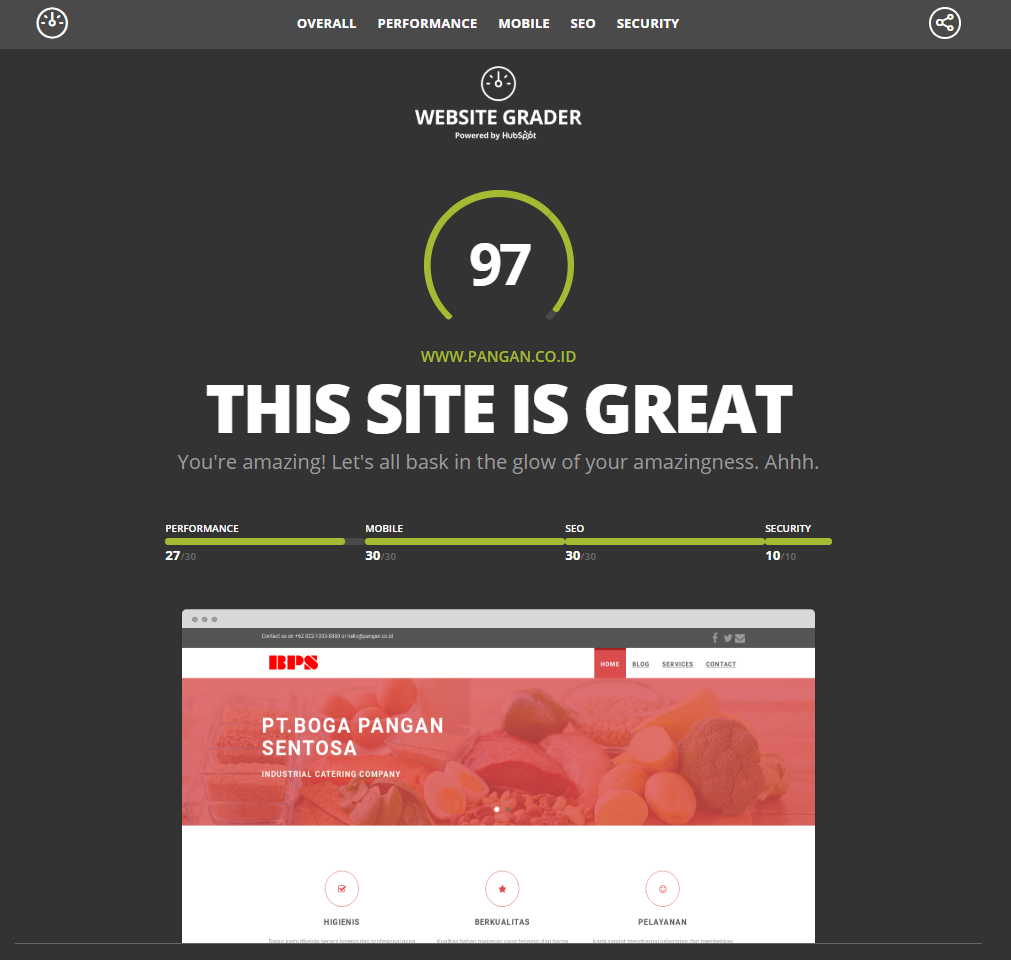
\includegraphics[width=10cm]{img/scr-website-grader.png}
    \caption{Standar nilai Performa \emph{website} pangan.co.id.}
    \label{gambar:scr-website-grader}
    \end{center}
\end{figure}

Dikarenakan penulis tidak ahli dalam bidang security maka penulis menggunakan 
online tools site checker security dan malware. Sucuri merupakan \emph{website} checker untuk 
mengetahui keamaan dan malware pada \emph{website} pangan.co.id. Hasil dari \emph{website} checker 
bahwa \emph{website} pangan.co.id tidak ditemukan malware, tidak adanya injected spam, 
tidak ada defacement, dan tidak ada internal error.didengan kata lain low security risk. 
Tidak adanya ancaman dari keamanan \emph{website}.

\begin{figure}[htbp]
    \begin{center}
    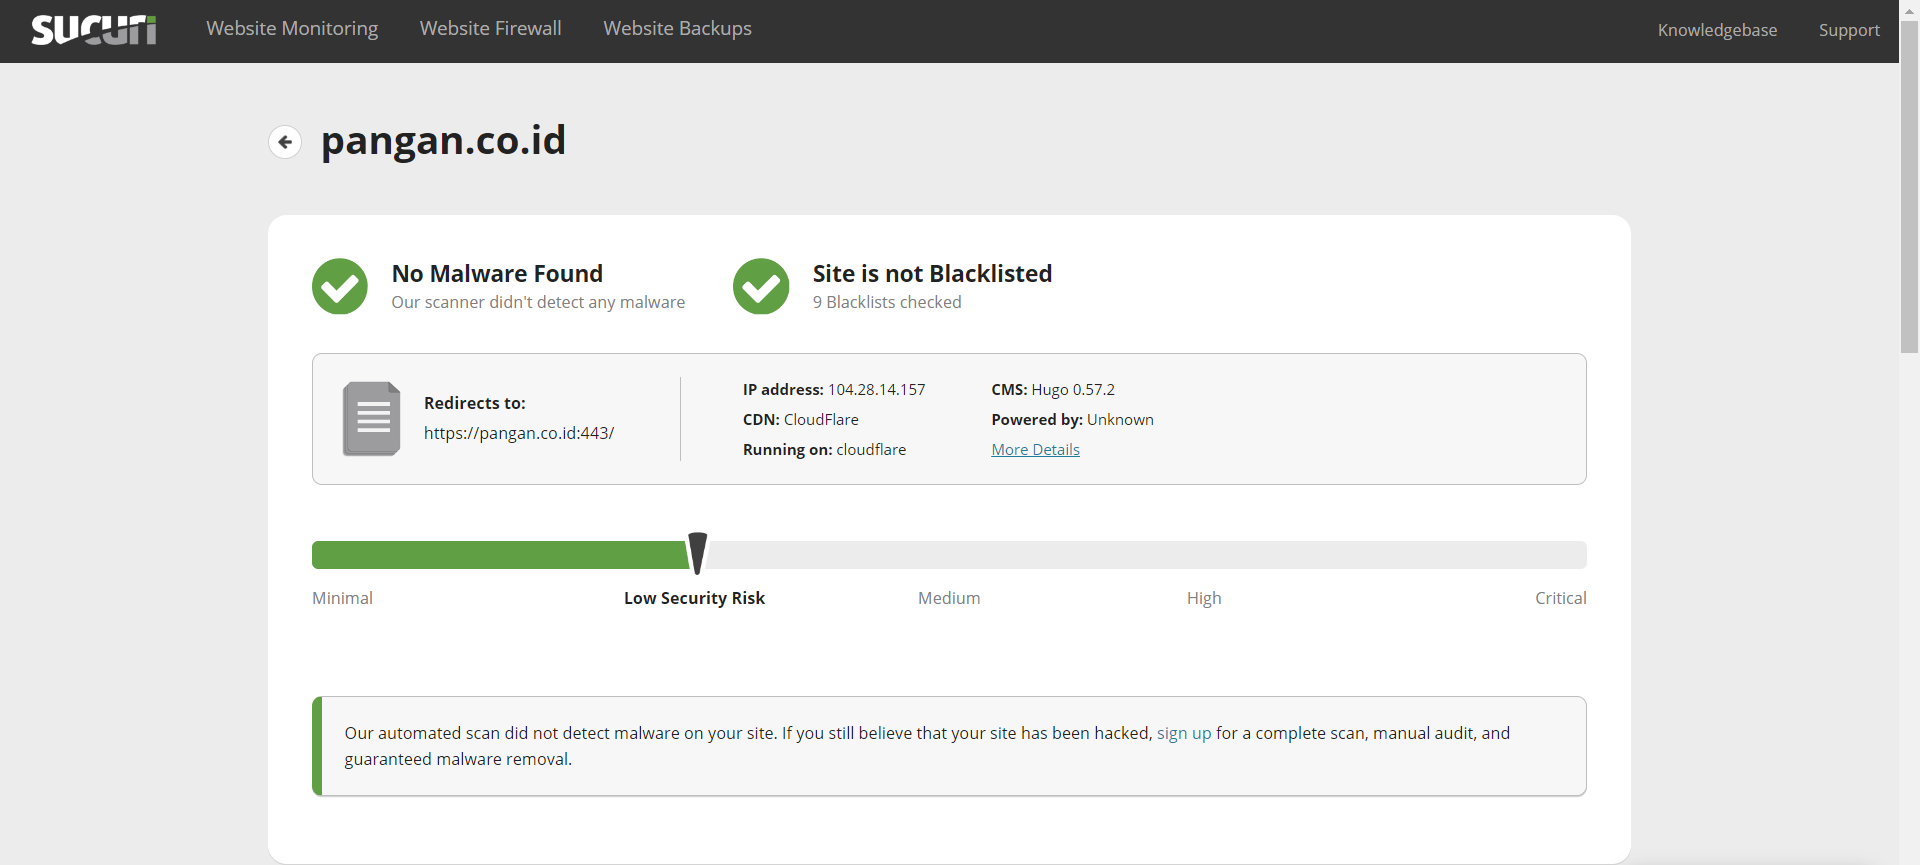
\includegraphics[width=10cm]{img/scr-suculi.png}
    \caption{Standar nilai keamanan dan malware checker}
    \label{gambar:scr-sucuri}
    \end{center}
\end{figure}

\pagebreak
Timeline kerja magang yang dilakukan penulis selama empat belas minggu serperti pada tabel 3.3

% Please add the following required packages to your document preamble:
% \usepackage{multirow}
\begin{table}[!htbp]
    \caption{Timeline Kerja Magang}
    \begin{tabular}{|l|l|l|l|l|l|l|l|l|l|l|l|l|l|l|l|}
    \hline
    \multicolumn{1}{|c|}{\multirow{2}{*}{No.}} & \multicolumn{1}{c|}{\multirow{2}{*}{Kegiatan}} & \multicolumn{14}{c|}{Minggu Ke}                            \\ \cline{3-16} 
    \multicolumn{1}{|c|}{}                     & \multicolumn{1}{c|}{}                          & 1 & 2 & 3 & 4 & 5 & 6 & 7 & 8 & 9 & 10 & 11 & 12 & 13 & 14 \\ \hline
    1                                          & Studi Literatur                                & x & x & x & x & x & x & x & x & x & x  & x  & x  & x  & x  \\ \hline
    2                                          & Requirement                                    & x & x &   &   &   &   & x &   &   &    &    &    &    &    \\ \hline
    3                                          & Instalasi dan setting-up                       &   & x & x &   &   &   &   &   &   &    &    &    &    &    \\ \hline
    4                                          & Implementasi                                   &   &   &   & x & x & x & x & x & x & x  &    &    &    &    \\ \hline
    5                                          & Testing                                        &   &   &   &   &   &   &   &   &   & x  & x  & x  & x  &    \\ \hline
    6                                          & Presentasi                                     &   &   & x &   &   & x &   &   & x &    &    & x  & x  &    \\ \hline
    7                                          & Dokumentasi                                    &   &   &   &   &   &   &   &   &   &    &    &    &    & x  \\ \hline
    \end{tabular}
    \end{table}


\subsection{Uraian Pelaksanaan Kerja Magang}

\subsubsection{Rancangan \emph{website}}
Gambaran sederhana yang dilakukan pengguna pada \emph{website} profil perusahaan dengan melihat halaman utama, 
blog, services dan contact us. \emph{website} profil perusahaan merupakan representasi 
perusahaan yang berisi informasi lengkap mengenai perusahaan dalam bentuk digital. 
Hal ini  memberi kesempatan bagi siapapun untuk mengakses dan menjadi nilai yang baik untuk masa depan perusahaan. 
Perancangan \emph{website} profil perusahaan akan dijelaskan lebih detail pada diagram arsitektur, 
menu hierarki diagram \emph{website} dan diagram use casee dan diagram arsitektur.

\subsubsection{Diagram Arsitektur}
Ruang lingkup dari \emph{website} profil perusahaan terdapat 3 linux container yaitu Hugo, 
Jupyter-notebook, dan traefik.  Traefik adalah proxy server dalam level micro-service 
untuk mengatur balance slot dan port forward. Ketiga container tersebut menggunakan kernel 
yang sama yaitu pada kernel Host OS. Traefik membuka akses port 80 (HTTP) dan 443 (HTTPS) ke 
jaringan agar dapat diakses oleh publik. Sedangkan Hugo dan jupyter memiliki internal network  
yang diatur oleh traefik 

Jupyter-notebook merupakan wadah untuk admin mengubah, menambah, menghapus konten. 
Memudahkan admin karena ‘wysiwyg’ what you see is what you get.\\

\begin{figure}[htbp]
    \begin{center}
    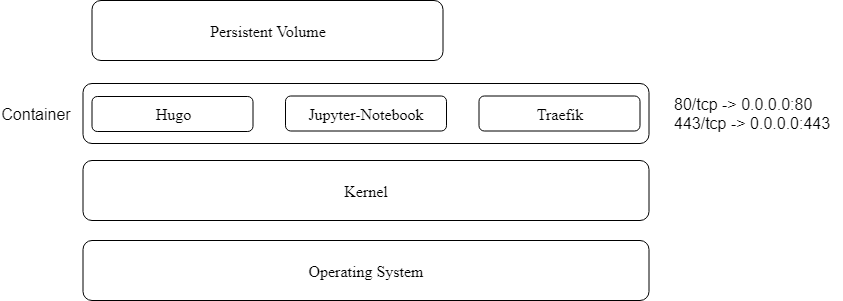
\includegraphics[width=15cm]{img/diag-arsitektur.png}
    \caption{Diagram Arsitektur}
    \label{gambar:diag-arsitektur}
    \end{center}
\end{figure}

\pagebreak
\subsubsection{Menu Hierarki Diagram \emph{website}}
\emph{website} profil perusahaan memiliki beberapa menu utama yang terdapat pada navigation bar. 
Menu utama berfungsi untuk memudahkan user untuk  berpindah halaman. 
Menu utama terbagi menjadi 4 yaitu Home, Blogs, Services dan Contact Us. 
Menu home memiliki konten nilai perusahaan, testimoni dari pelanggan, 
terdapat tombol untuk mengunduh company profile, recent post dari blog, dan client. 
Pada menu blogs, yang berisikan artikel-artikel. Menu Services berisikan uraian layanan yang 
ditawarkan perusahaan. 
Menu Contact Us berisikan informasi kontak perusahaan pada halaman ini pengunjung dapat mengisi 
form atau menghubungi nomor yang tertera pada halaman tersebut.

\begin{figure}[htbp]
    \begin{center}
    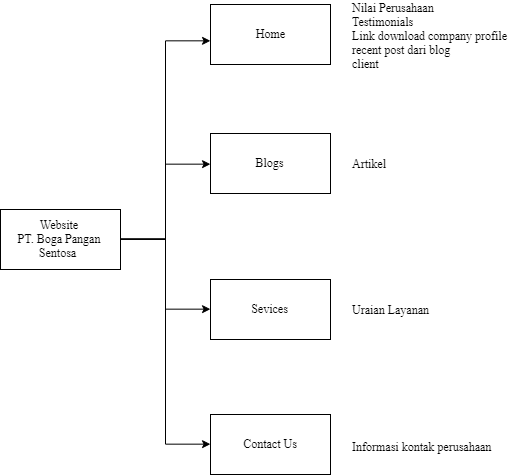
\includegraphics[width=12cm]{img/diag-menu.png}
    \caption{Hirarki Menu Diagram \emph{website}}
    \label{gambar:diag-menu}
    \end{center}
\end{figure}

\pagebreak
\subsubsection{Diagram Use Case}

Diagram use case merupakan pemodelan untuk menggambarkan kelakuan sistem yang akan dibuat. 
Diagram use case mendeskripsikan sebuah interaksi antara satu atau lebih aktor dengan sitem yang akan dibuat[4]. 
Diagram ini digunakan untuk mengetahui fungsi apa saja yang ada di dalam suatu sistem dan siapa saja yang berhak 
menggunakan fungsi tersebut[4]. Pada diagram Use Case, terdapat 2 aktor yaitu User dan Admin. User pengguna 
dapatmemiliki akses Read Only (RO) seperti:  melihat informasi mengenai PT. BPS, melihat layanan PT.BPS, melihat 
artikel blog, melihat informasi contact service. Sedangkan Admin memiliki kewenangan untuk dapat melakukan Create, 
Read, Update dan Detete (CRUD) terhadap suatu konten. 

\begin{figure}[htbp]
    \begin{center}
    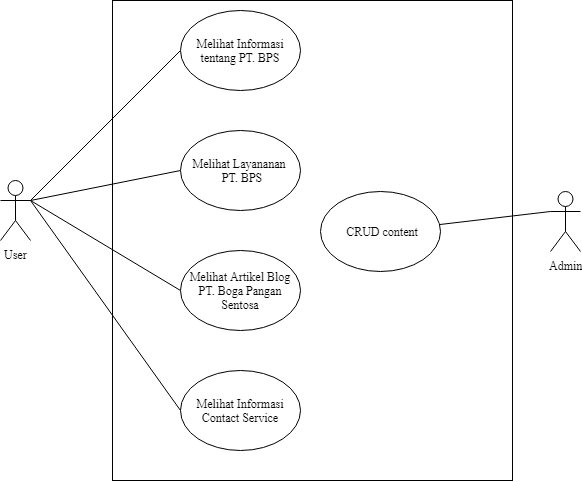
\includegraphics[width=12cm]{img/diag-usecase.png}
    \caption{Diagram Use Case}
    \label{gambar:diag-usecase}
    \end{center}
\end{figure}

\subsubsection{Implementasi \emph{website}}
Admin dapat mengunakan alamat situs note.pangan.co.id 
dimana \emph{jupyter notebook} di \emph{install}. yang berguna 
untuk membuang atau menambahkan konten.  
Admin menuju ke folder content > blogs untuk menambahkan artikel pada halaman blogs. 
Admin harus mengetahui bagaimana cara menulis artikel pada \emph{markdown} (md). 
Penulis memberikan panduan cara menulis artikel dengan format (md). 

\begin{figure}[htbp]
    \begin{center}
    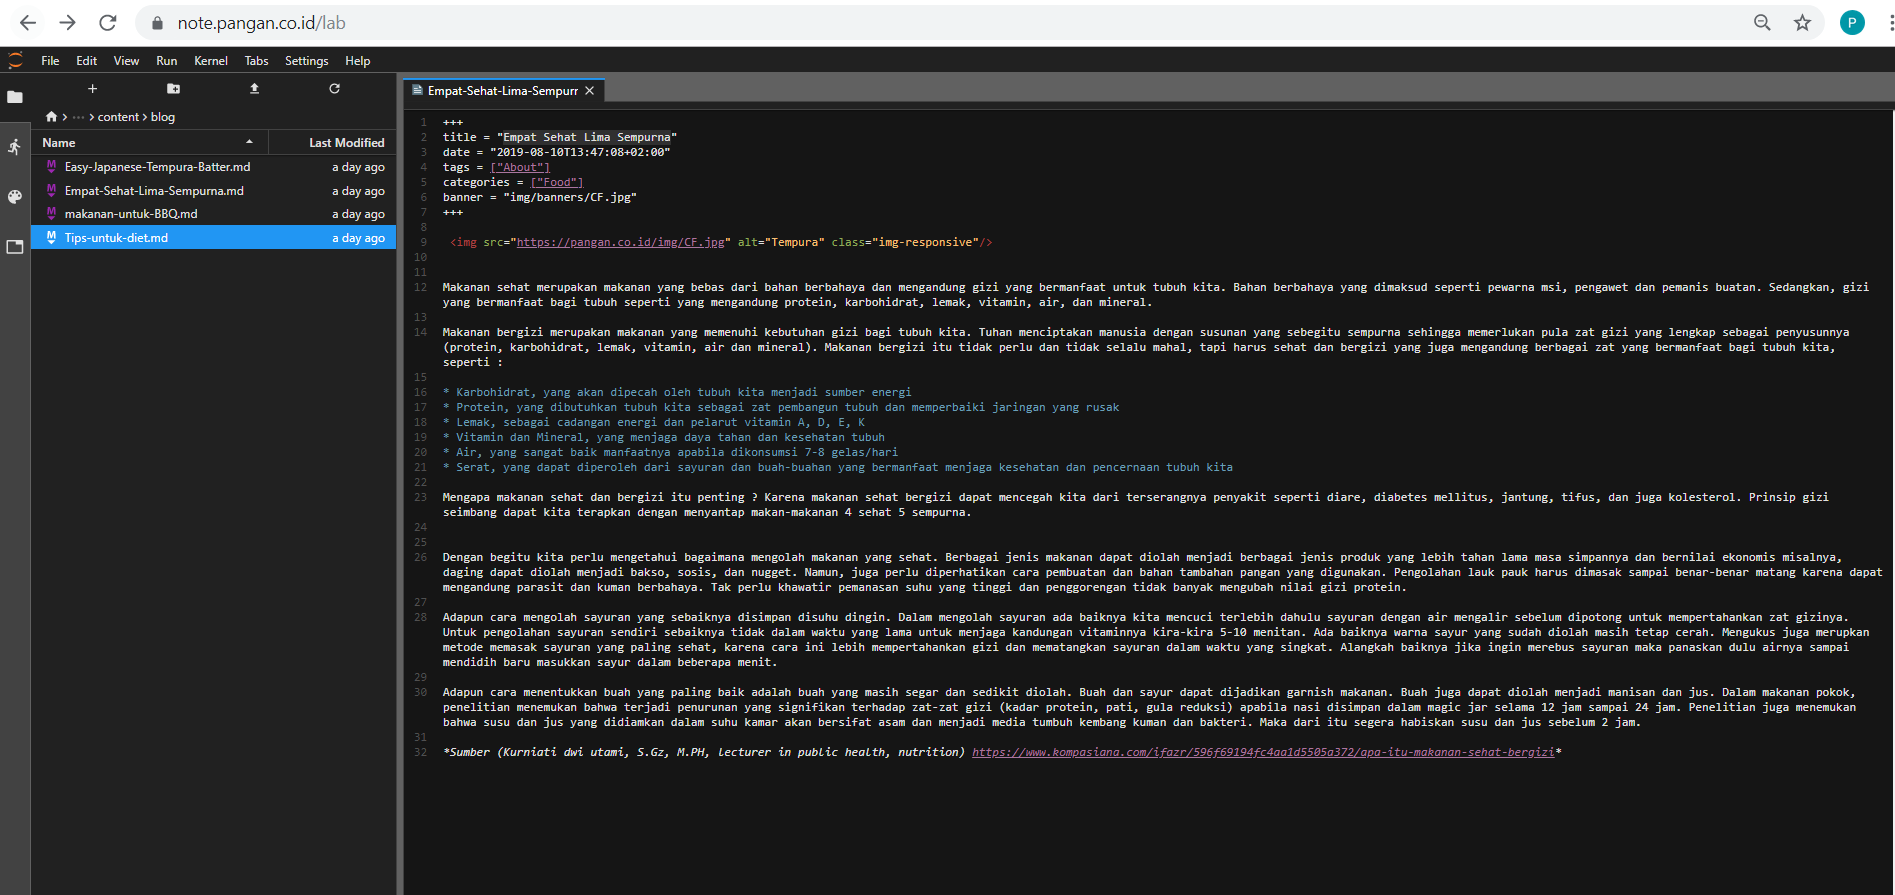
\includegraphics[width=12cm]{img/scr-adm-1.png}
    \caption{Jupyter Notebook section blog}
    \label{gambar:scr-adm-1}
    \end{center}
\end{figure}


Berikut Tampilan folder listing yang dapat diakses oleh admin. Untuk mengubah suatu konten, 
Admin harus mengakses folder “content” lalu terdapat folder “blog”.

\begin{figure}[htbp]
    \begin{center}
    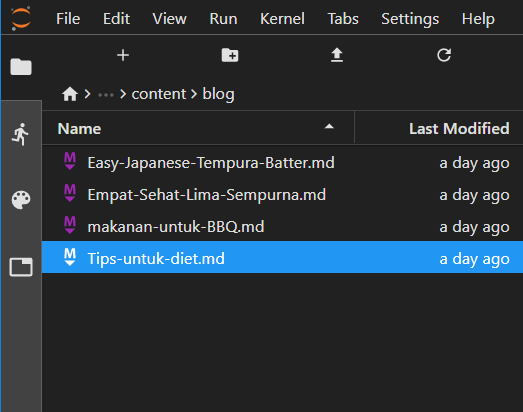
\includegraphics[width=7cm]{img/scr-adm-2.png}
    \caption{Folder Listing}
    \label{gambar:scr-adm-2}
    \end{center}
\end{figure}


\begin{figure}[htbp]
    \begin{center}
    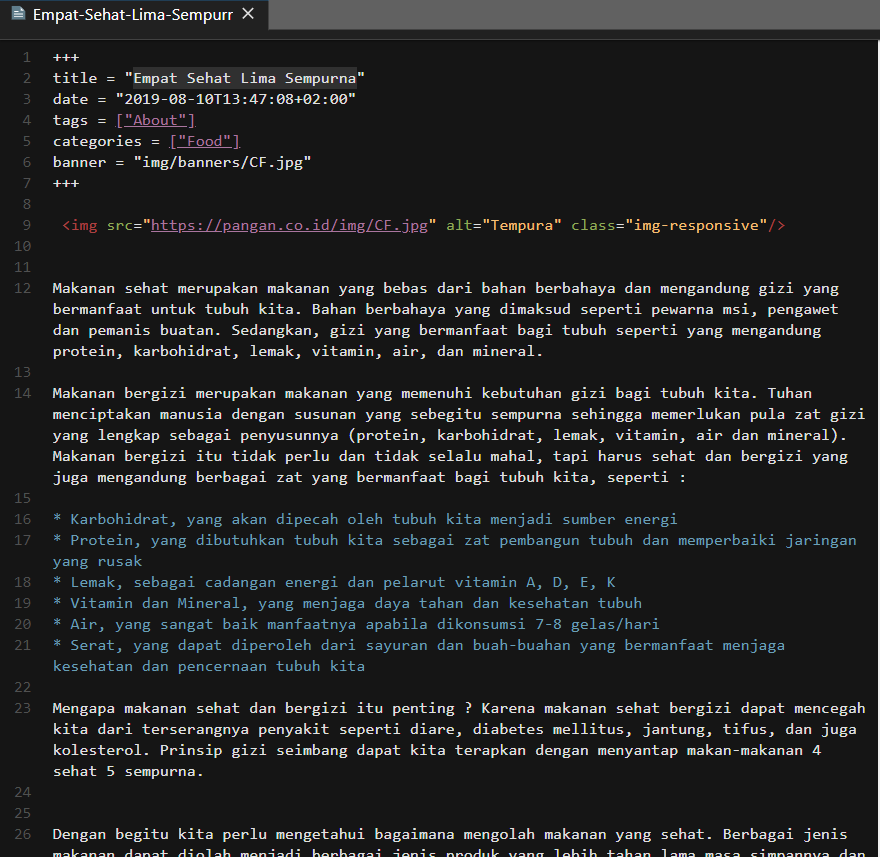
\includegraphics[width=8cm]{img/scr-adm-3.png}
    \caption{Tampilan edit dengan format markdown}
    \label{gambar:scr-adm-3}
    \end{center}
\end{figure}

Selain menambah artikel pada blog admin dapat mengubah lainnya seperti uraian pada service, 
kontak perusahaan, atau menambah testimonial dari pelanggan.

\begin{figure}[htbp]
    \begin{center}
    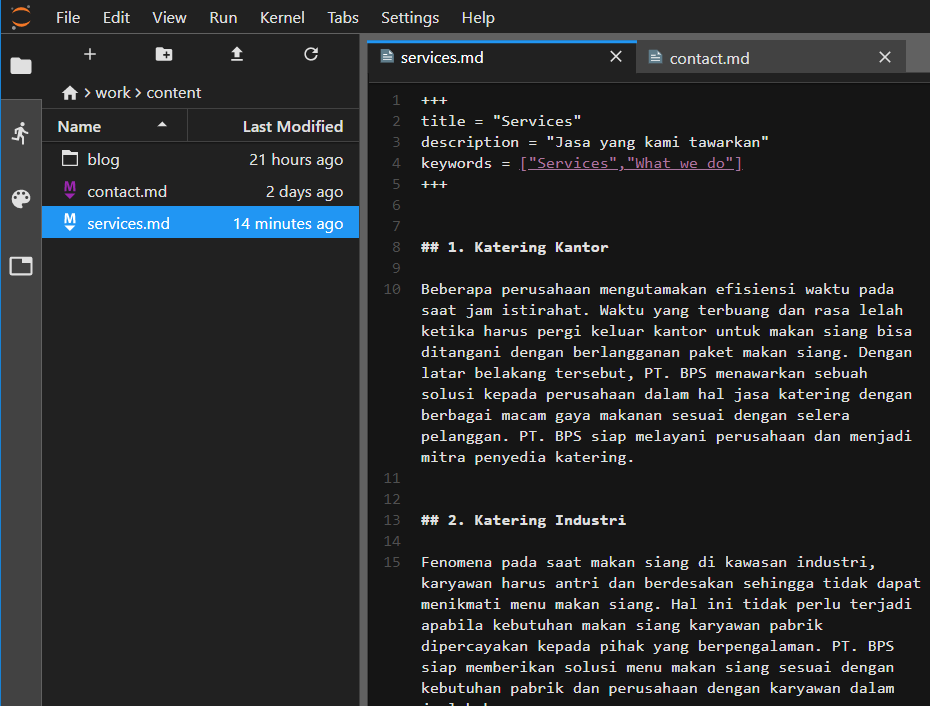
\includegraphics[width=8cm]{img/scr-adm-4.png}
    \caption{Tampilan edit services.md dan contact.md}
    \label{gambar:scr-adm-4}
    \end{center}
\end{figure}


Pada \emph{website} profil perusahaan, halaman utama terdiri dari carousel, nilai perusahaan, 
terstimonial, banner, recent post, client, footer. Bagian navigation bar berisi Home, 
Blog, Service dan Contact. Testimoni dari pelanggan yang sudah berlangganan dengan 
PT. BPS. Banner yang tertera pada halaman utama. Jika pengguna ingin mengetahui 
PT. BPS lebih lanjut, pengguna dapat menekan tombol 
“Check other homepages” yang akan mengunduh company profile. 


% Tampilan Webiste
%
%

\begin{figure}[htbp]
    \begin{center}
    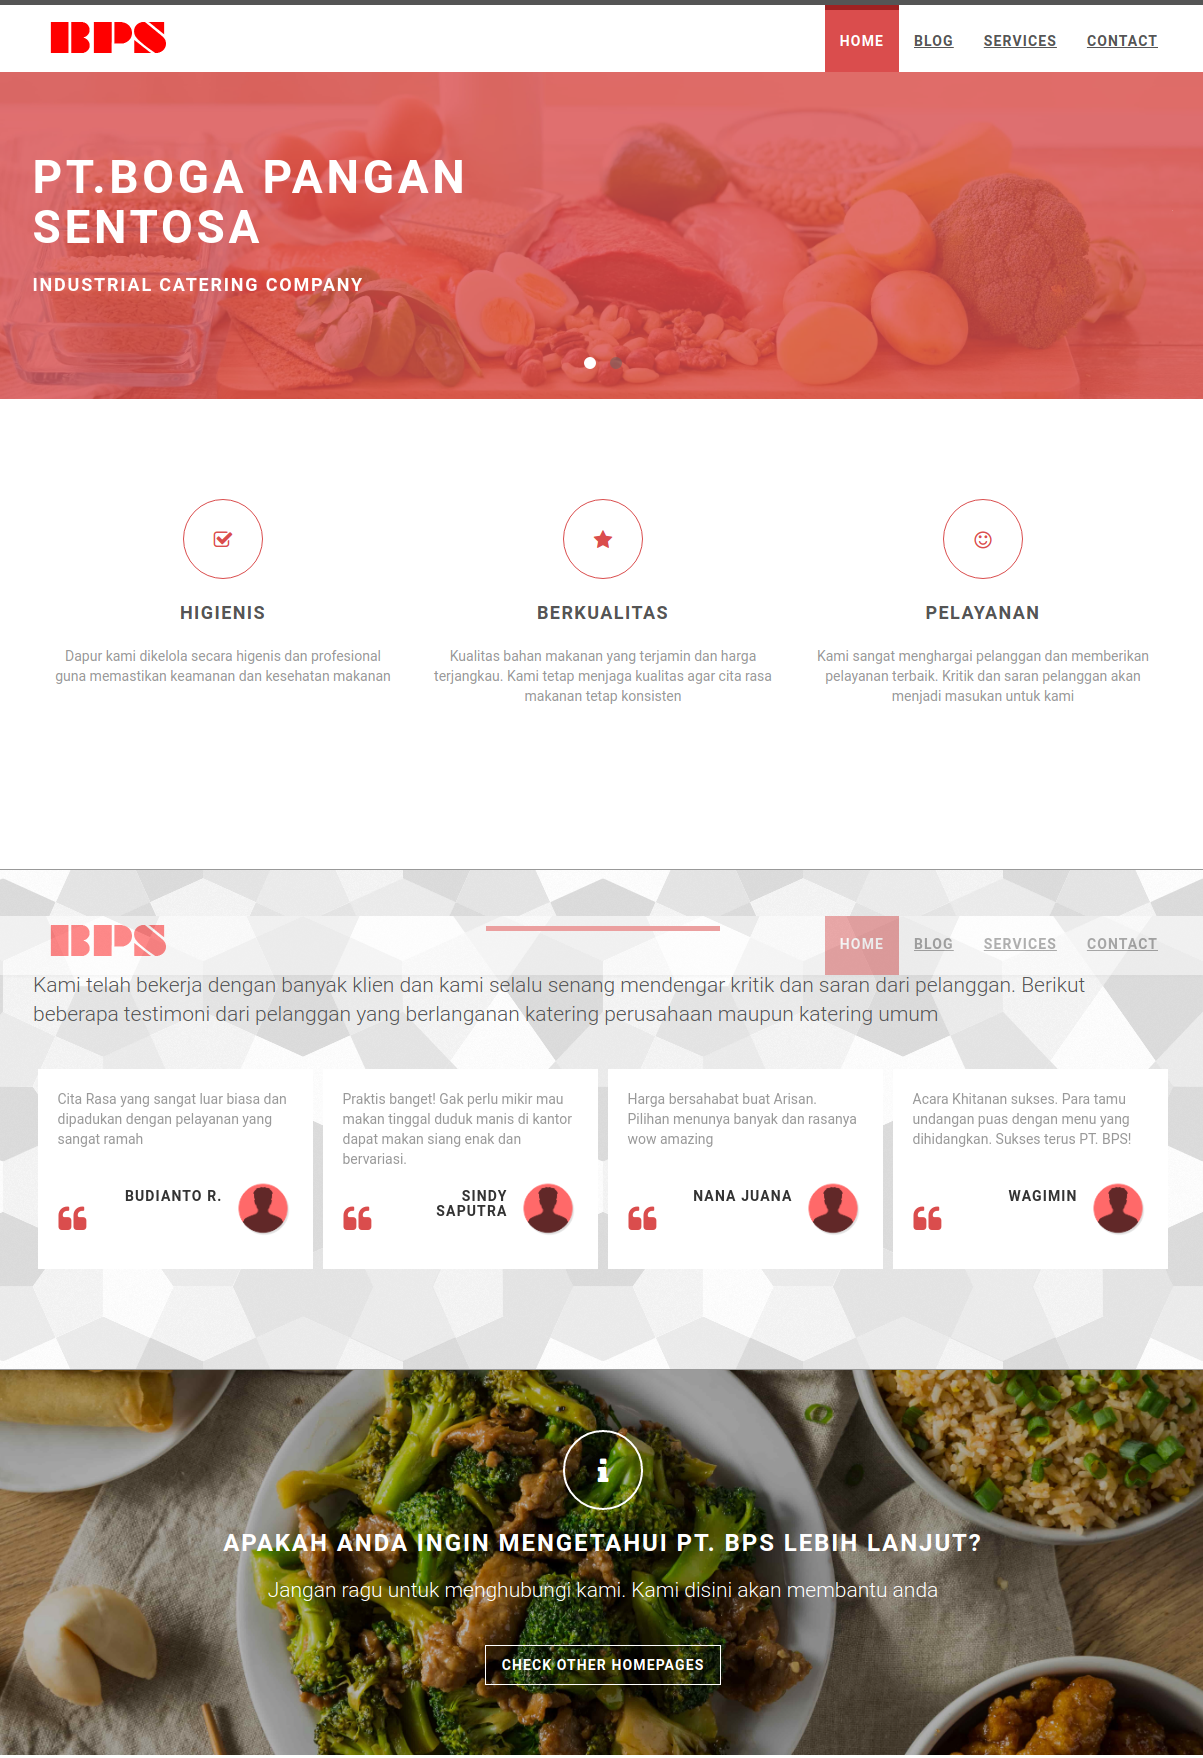
\includegraphics[width=7cm]{img/scr-website-1.png}
    \caption{Halaman Utama}
    \label{gambar:scr-website-1}
    \end{center}
\end{figure}

Pada recent post menampilkan empat artikel terakhir yang ditambahkan oleh admin. 
User dapat mengarahkan kursor ke gambar atau tombol continue reading,  
akan mebuka halaman blog. Bagian Our Clients terdapat beberapa logo perusahaan yang menjadi 
pelanggan dan merasakan hidangan dan pelyanan yang  diberika oleh 
PT. BPS. Footer terdapat pada setiap halaman, 
Footer terbagi menjadi beberapa bagian yang menampilkan about us secara singkat, 
recent posts, contact, dan copyright.

% Blog
%
%

Halaman ini memuat artikel yang berkategori tips, resep, dan makanan. 
Blogs dibuat dengan harapan selain melihat company profile dari BPS, 
juga dapat melihat artikel-artikel. Side menu yang berisikan search, 
categories, dan tags yang memudahkan user dalam pencaharian artikel yang ingin dibaca.

\begin{figure}[htbp]
    \begin{center}
    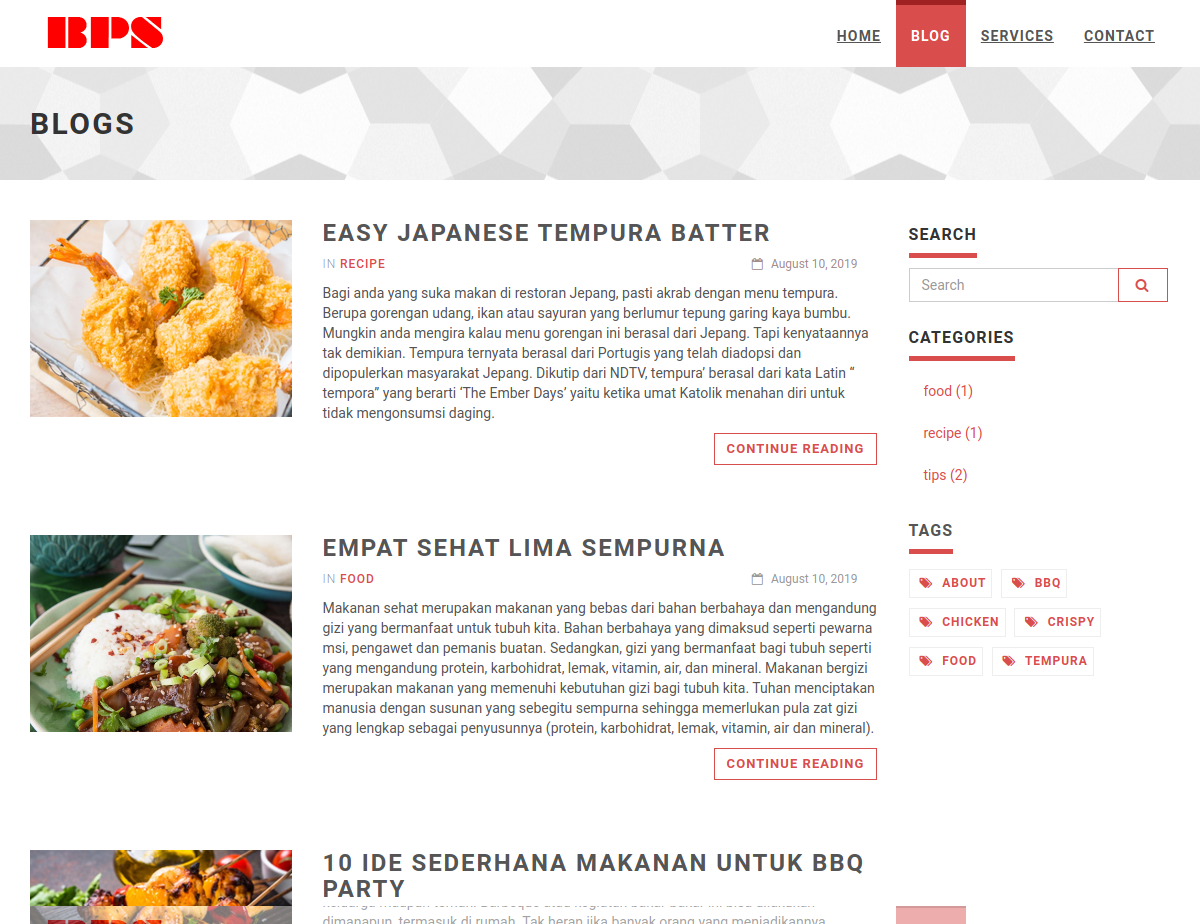
\includegraphics[width=8cm]{img/scr-website-blog.png}
    \caption{Halaman Blog}
    \label{gambar:scr-website-blog}
    \end{center}
\end{figure}


Halaman services yang berisikan uraian pelayanan yang ditawarkan perusahaan 
PT. BPS menawarkan katering kantor, karting industry dan katering umum. Calon 
pelanggan dapat memilih sesuai dengan kebutuhan dari perusahaan. 
Jika calon pelanggan ingin mengetahui lebih lanjut dapat menjutu navigation bar dan menekan tombol contact

\begin{figure}[htbp]
    \begin{center}
    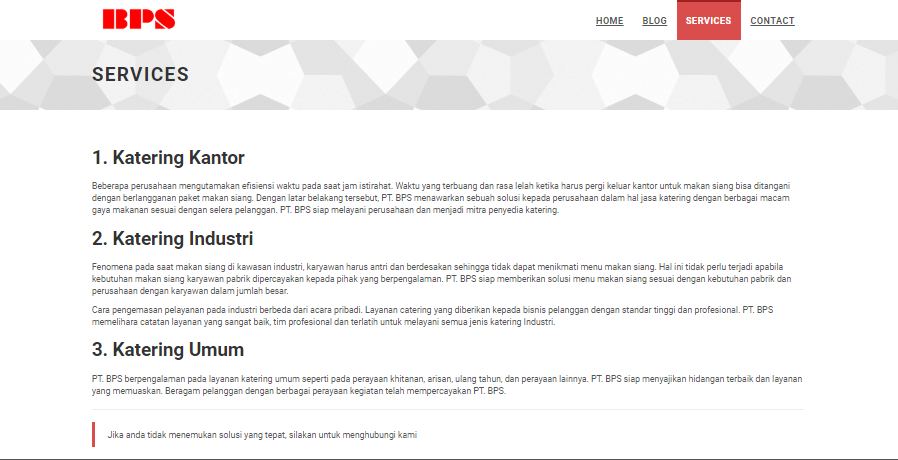
\includegraphics[width=8cm]{img/scr-website-service.png}
    \caption{Halaman Service}
    \label{gambar:scr-website-service}
    \end{center}
\end{figure}

Halaman contact terdiri dari contact form, telepon, dan alamat perusahaan. 
Calon pelanggan yang tertarik dengan layanan yang diberikan oleh perusahaan dapat langsung mengisi 
contact form dan akan langsung terkirim \\ke hello@pangan.co.id.  
Calon pelanggan mengunjungi alamat perusahaan atau menelfon di nomor layanan yang tertera.

\begin{figure}[htbp]
    \begin{center}
    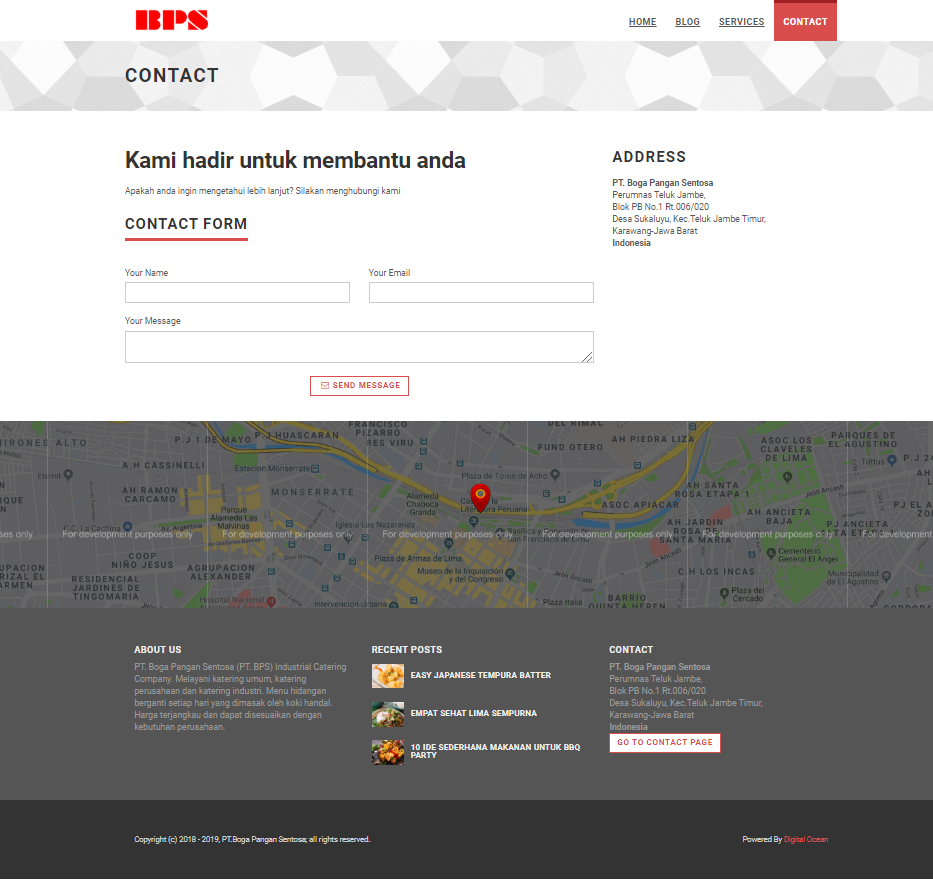
\includegraphics[width=5cm]{img/scr-website-contact.png}
    \caption{Halaman kontak}
    \label{gambar:scr-website-contact}
    \end{center}
\end{figure}

\subsection{Kendala yang ditemukan}

Pada proses pembuatan \emph{website} profil perusahaan terdapat kendala yang ditemukan 
seperti sulitnya mengisi konten \emph{website} dikarenakan minimnya informasi dan 
dokumentasi yang layak dari perusahaan. Selain itu kendala yang lain yaitu user acceptance. 
User Acceptance adalah tahap akhir pada testing yang 
dijalankan untuk mengetahui apakah masih terdapat kecacatan pada \emph{website} yang dikembangkan.

\subsection{Solusi atas kendala yang ditemukan}
Solusi untuk menyelesaikan kendala 3.4 yaitu dengan \emph{gathering} data perusahaan dan 
menampilkam beberapa dokumentasi yang layak. 
Untuk menyelesaikan masalah \emph{user acceptance} yaitu melakukan \emph{survey} dengan melakukan wawancara. 